\documentclass[iop,apj,twocolumn,twocolappendix,numberedappendix]{emulateapj}
\usepackage{apjfonts}
\usepackage{multirow}
\usepackage{textcomp}
\usepackage{amsmath}
\usepackage{microtype}
\usepackage{subfigure}
\usepackage{xcolor,ulem}
\usepackage[breaklinks=true]{hyperref}

%@arxiver{mass_boxes,Fig_mass_SNR,spin_cred_regions}

\begin{document}

\title{Parameter estimation on gravitational waves from neutron-star binaries with spinning components}

\slugcomment{Submitted to ApJ}

\input{"authorlist.tex"}

\shorttitle{PE on GWs from BNSs with spinning components}
\shortauthors{Farr et al.}

\input{"abstract.tex"}

\input{"introduction.tex"}

\input{"sources.tex"}

\input{"spinning_analysis.tex"}

\input{"mass_estimates.tex"}

\begin{figure*}
  \centering
  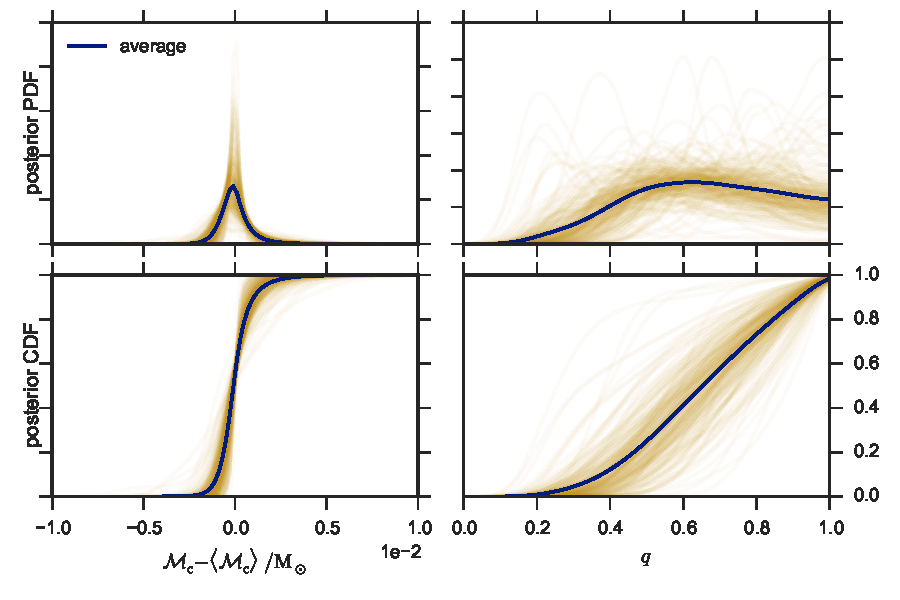
\includegraphics[width=1.6\columnwidth]{figures/spinning-masses/quad_mass_grid}
  \caption{\protect\label{fig:spinPDFcred} The distribution of one-dimensional marginalized posterior probability density functions (PDFs) of spin magnitudes of the more and less massive components ($\chi_1$ and $\chi_2$, respectively) for all $250$ simulated sources. Shaded regions show the $90\%$ credible boundaries for the spin distributions of the population, and the solid lines show the average of each PDF.  The posteriors have very consistent morphology and span the majority of the prior range.  The spin of the most massive component is typically slightly more constrained toward low values, but even a maximal spin of $\chi_1 = 1$ is rarely ruled out.
  } 
\end{figure*}

\begin{figure}
  \centering
  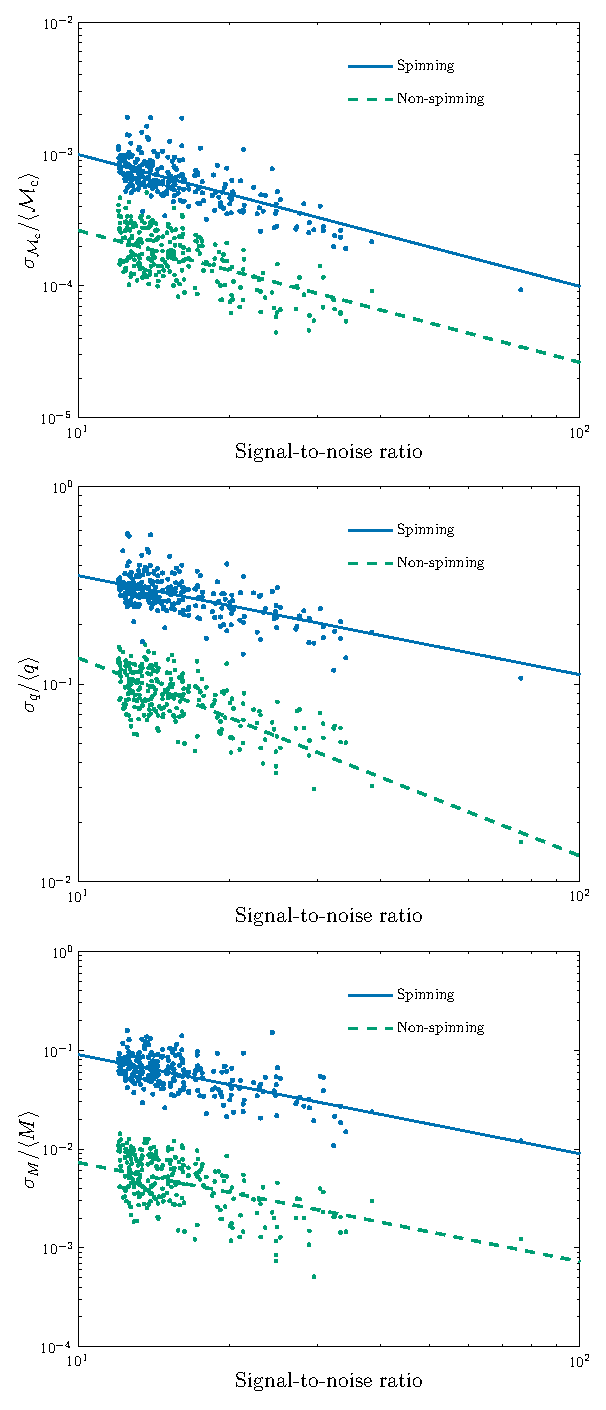
\includegraphics[width=0.85\columnwidth]{figures/Fig_mass_SNR/Fig_mass_SNR}
  \caption{\protect\label{fig:spinPDFcred} The distribution of one-dimensional marginalized posterior probability density functions (PDFs) of spin magnitudes of the more and less massive components ($\chi_1$ and $\chi_2$, respectively) for all $250$ simulated sources. Shaded regions show the $90\%$ credible boundaries for the spin distributions of the population, and the solid lines show the average of each PDF.  The posteriors have very consistent morphology and span the majority of the prior range.  The spin of the most massive component is typically slightly more constrained toward low values, but even a maximal spin of $\chi_1 = 1$ is rarely ruled out.
  } 
\end{figure}

\input{"spin_estimates.tex"}

\begin{figure}
  \centering
  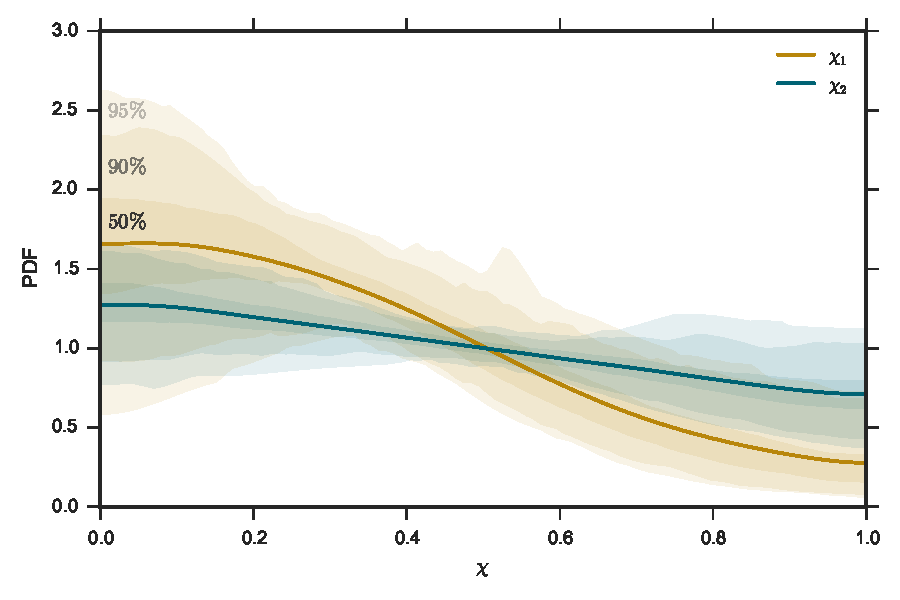
\includegraphics[width=0.95\columnwidth]{figures/spin_cred_regions/spin_cred_regions}
  \caption{\protect\label{fig:spinPDFcred} The distribution of one-dimensional marginalized posterior probability density functions (PDFs) of spin magnitudes of the more and less massive components ($\chi_1$ and $\chi_2$, respectively) for all $250$ simulated sources. Shaded regions show the $90\%$ credible boundaries for the spin distributions of the population, and the solid lines show the average of each PDF.  The posteriors have very consistent morphology and span the majority of the prior range.  The spin of the most massive component is typically slightly more constrained toward low values, but even a maximal spin of $\chi_1 = 1$ is rarely ruled out.
  } 
\end{figure}

\input{"spin_priors.tex"}

\begin{figure}
  \centering
  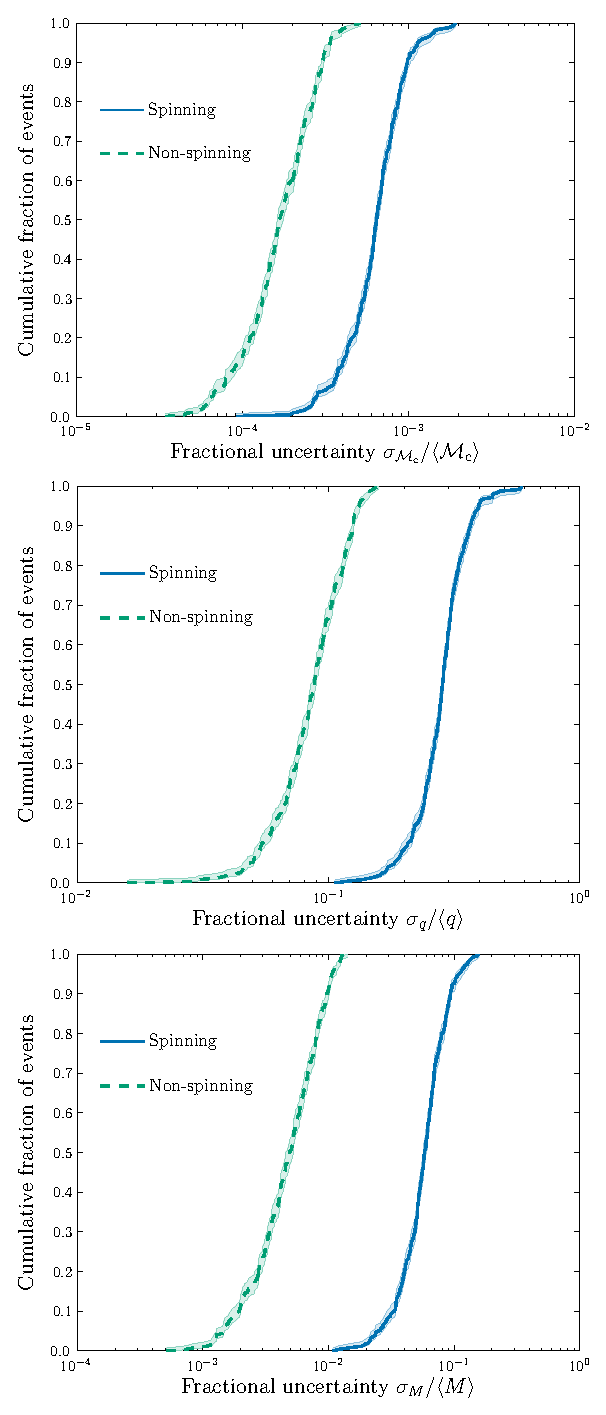
\includegraphics[width=0.85\columnwidth]{figures/Fig_mass_fractional/Fig_mass_fractional}
  \caption{\protect\label{fig:spinPDFcred} The distribution of one-dimensional marginalized posterior probability density functions (PDFs) of spin magnitudes of the more and less massive components ($\chi_1$ and $\chi_2$, respectively) for all $250$ simulated sources. Shaded regions show the $90\%$ credible boundaries for the spin distributions of the population, and the solid lines show the average of each PDF.  The posteriors have very consistent morphology and span the majority of the prior range.  The spin of the most massive component is typically slightly more constrained toward low values, but even a maximal spin of $\chi_1 = 1$ is rarely ruled out.
  } 
\end{figure}

\input{"component_masses.tex"}

\begin{figure}
  \centering
  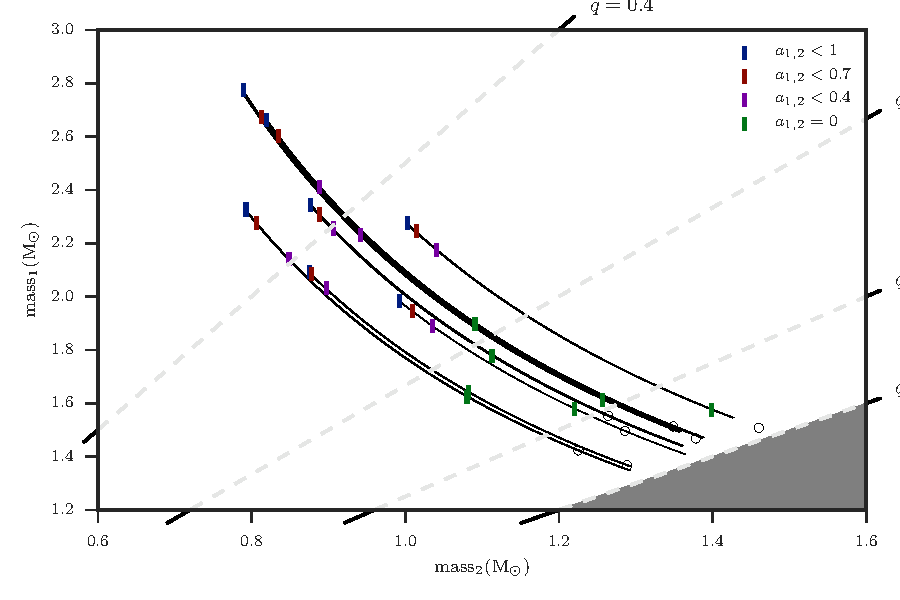
\includegraphics[width=1.0\columnwidth]{figures/compmasses/mass_boxes}
  \caption{\protect\label{fig:spinPDFcred} The distribution of one-dimensional marginalized posterior probability density functions (PDFs) of spin magnitudes of the more and less massive components ($\chi_1$ and $\chi_2$, respectively) for all $250$ simulated sources. Shaded regions show the $90\%$ credible boundaries for the spin distributions of the population, and the solid lines show the average of each PDF.  The posteriors have very consistent morphology and span the majority of the prior range.  The spin of the most massive component is typically slightly more constrained toward low values, but even a maximal spin of $\chi_1 = 1$ is rarely ruled out.
  } 
\end{figure}

\input{"mass_ratio.tex"}

\begin{figure}
  \centering
  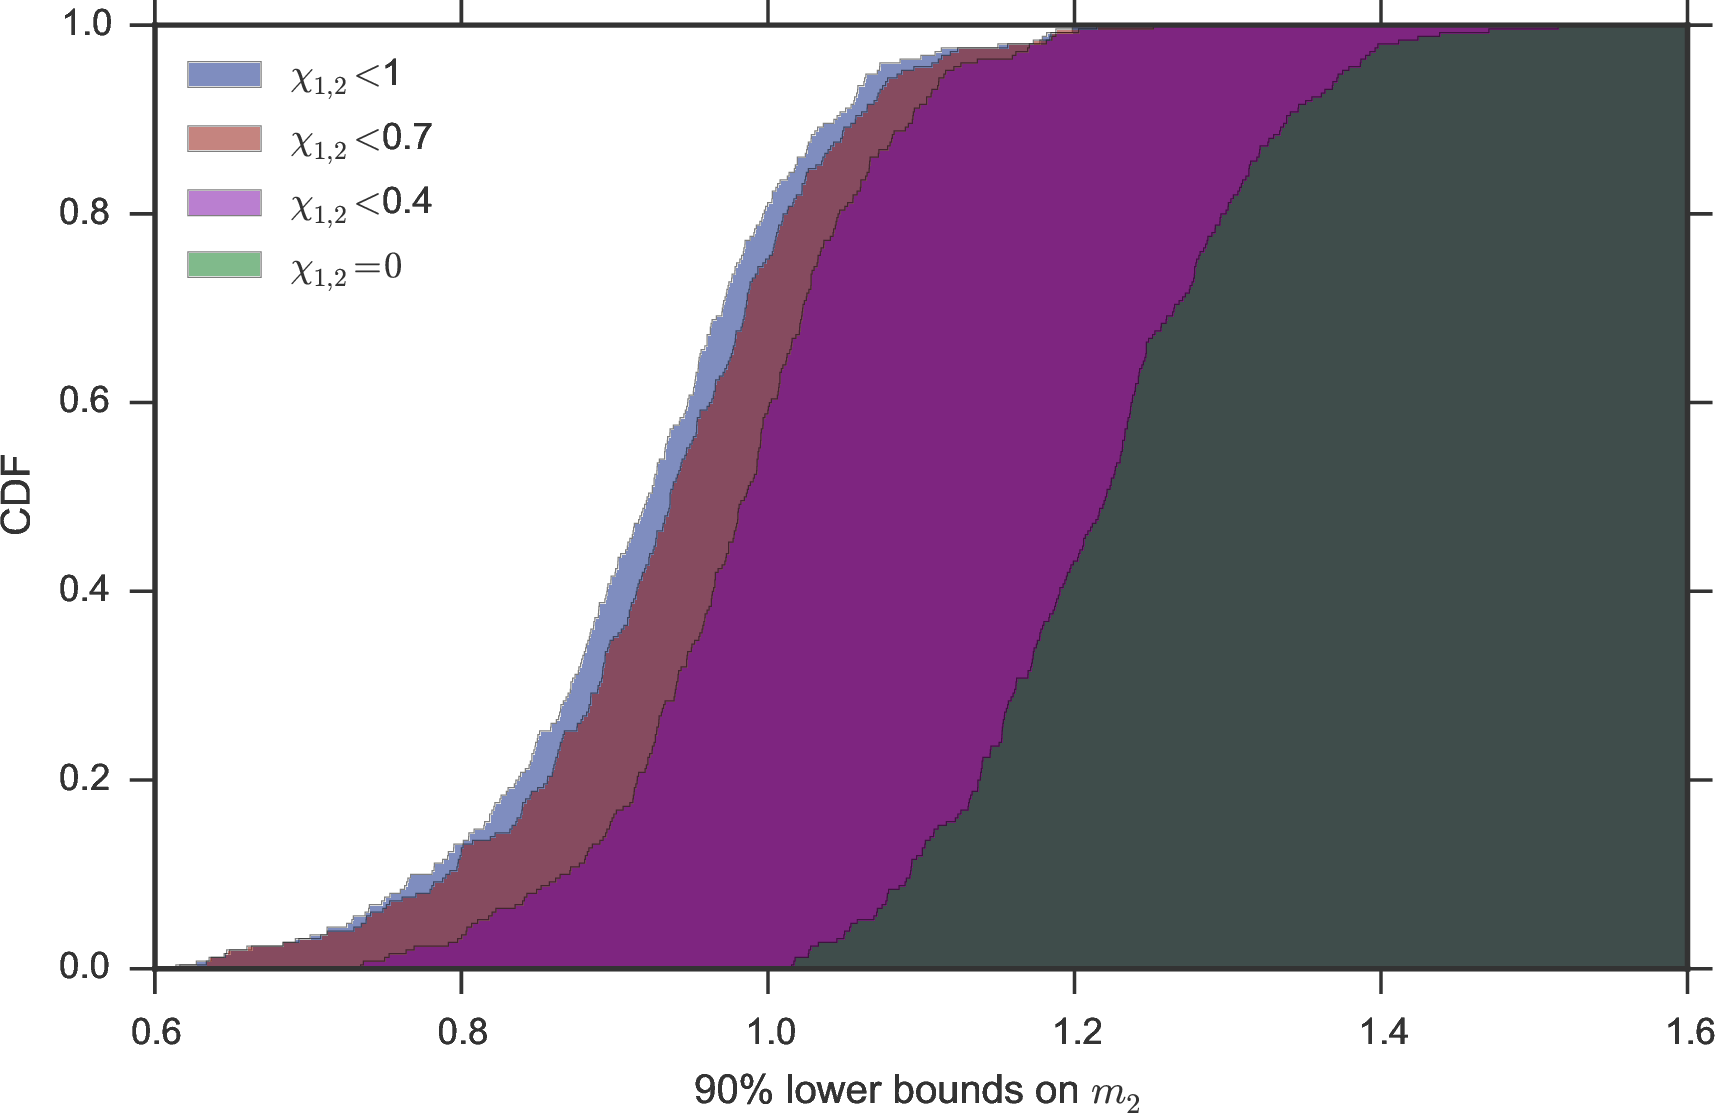
\includegraphics[width=0.95\columnwidth]{figures/mass-ratio/m2_cumulatives}
  \caption{\protect\label{fig:spinPDFcred} The distribution of one-dimensional marginalized posterior probability density functions (PDFs) of spin magnitudes of the more and less massive components ($\chi_1$ and $\chi_2$, respectively) for all $250$ simulated sources. Shaded regions show the $90\%$ credible boundaries for the spin distributions of the population, and the solid lines show the average of each PDF.  The posteriors have very consistent morphology and span the majority of the prior range.  The spin of the most massive component is typically slightly more constrained toward low values, but even a maximal spin of $\chi_1 = 1$ is rarely ruled out.
  } 
\end{figure}

\input{"sky_localization.tex"}

\begin{figure}
  \centering
  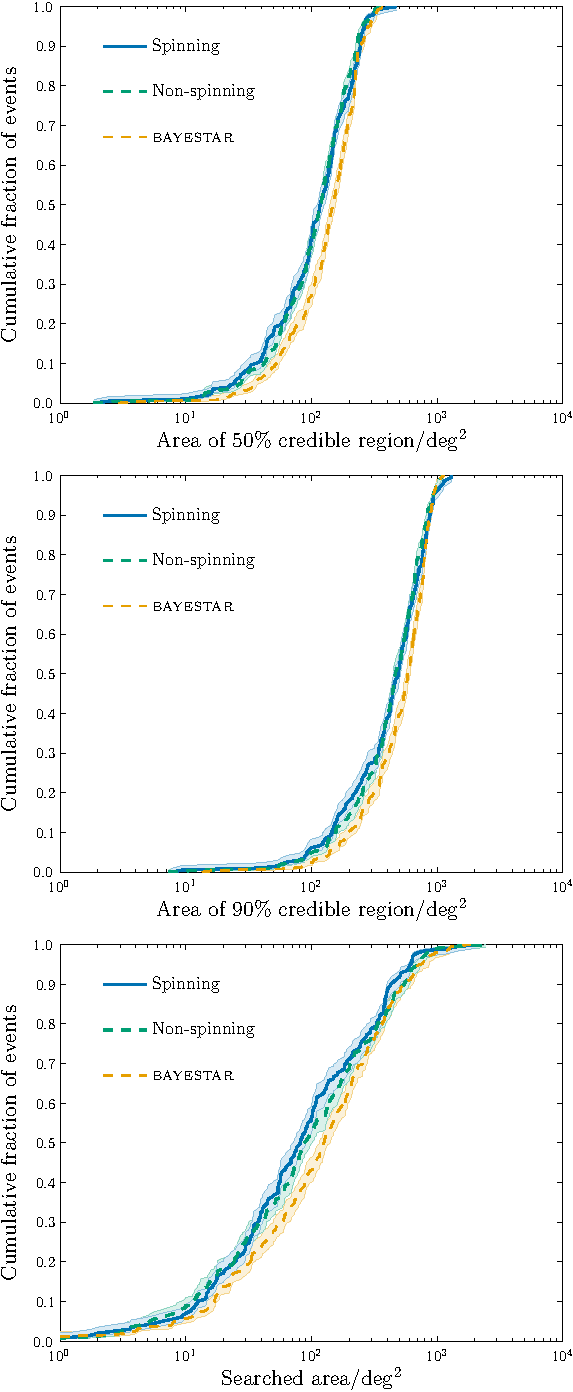
\includegraphics[width=0.85\columnwidth]{figures/Fig_3_sky_areas/Fig_3_sky_areas}
  \caption{\protect\label{fig:spinPDFcred} The distribution of one-dimensional marginalized posterior probability density functions (PDFs) of spin magnitudes of the more and less massive components ($\chi_1$ and $\chi_2$, respectively) for all $250$ simulated sources. Shaded regions show the $90\%$ credible boundaries for the spin distributions of the population, and the solid lines show the average of each PDF.  The posteriors have very consistent morphology and span the majority of the prior range.  The spin of the most massive component is typically slightly more constrained toward low values, but even a maximal spin of $\chi_1 = 1$ is rarely ruled out.
  } 
\end{figure}

\input{"run-by-run_skyareas.tex"}

\input{"paper-sky-ratio-table.tex"}

\input{"luminosity_distance.tex"}

\begin{figure*}
  \centering
  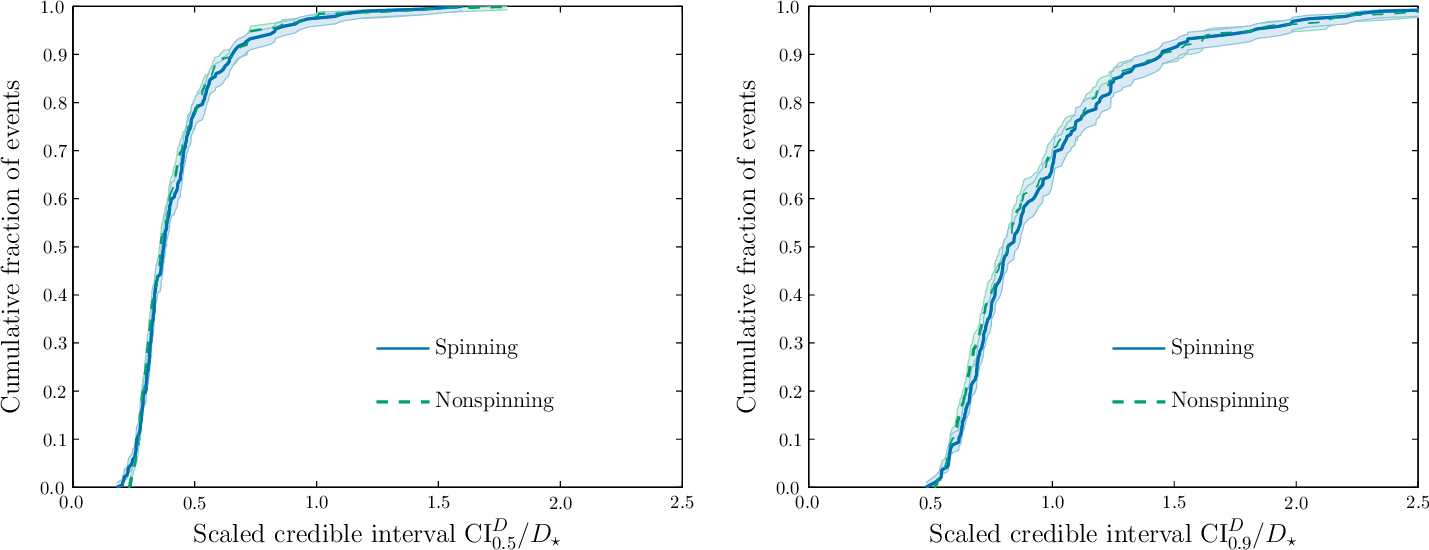
\includegraphics[width=1.7\columnwidth]{figures/Fig_spin_dist/Fig_spin_dist}
  \caption{\protect\label{fig:spinPDFcred} The distribution of one-dimensional marginalized posterior probability density functions (PDFs) of spin magnitudes of the more and less massive components ($\chi_1$ and $\chi_2$, respectively) for all $250$ simulated sources. Shaded regions show the $90\%$ credible boundaries for the spin distributions of the population, and the solid lines show the average of each PDF.  The posteriors have very consistent morphology and span the majority of the prior range.  The spin of the most massive component is typically slightly more constrained toward low values, but even a maximal spin of $\chi_1 = 1$ is rarely ruled out.
  } 
\end{figure*}

\input{"summary.tex"}

\input{"acknowledgements.tex"}

\input{"computational_cost.tex"}

\begin{figure}
  \centering
  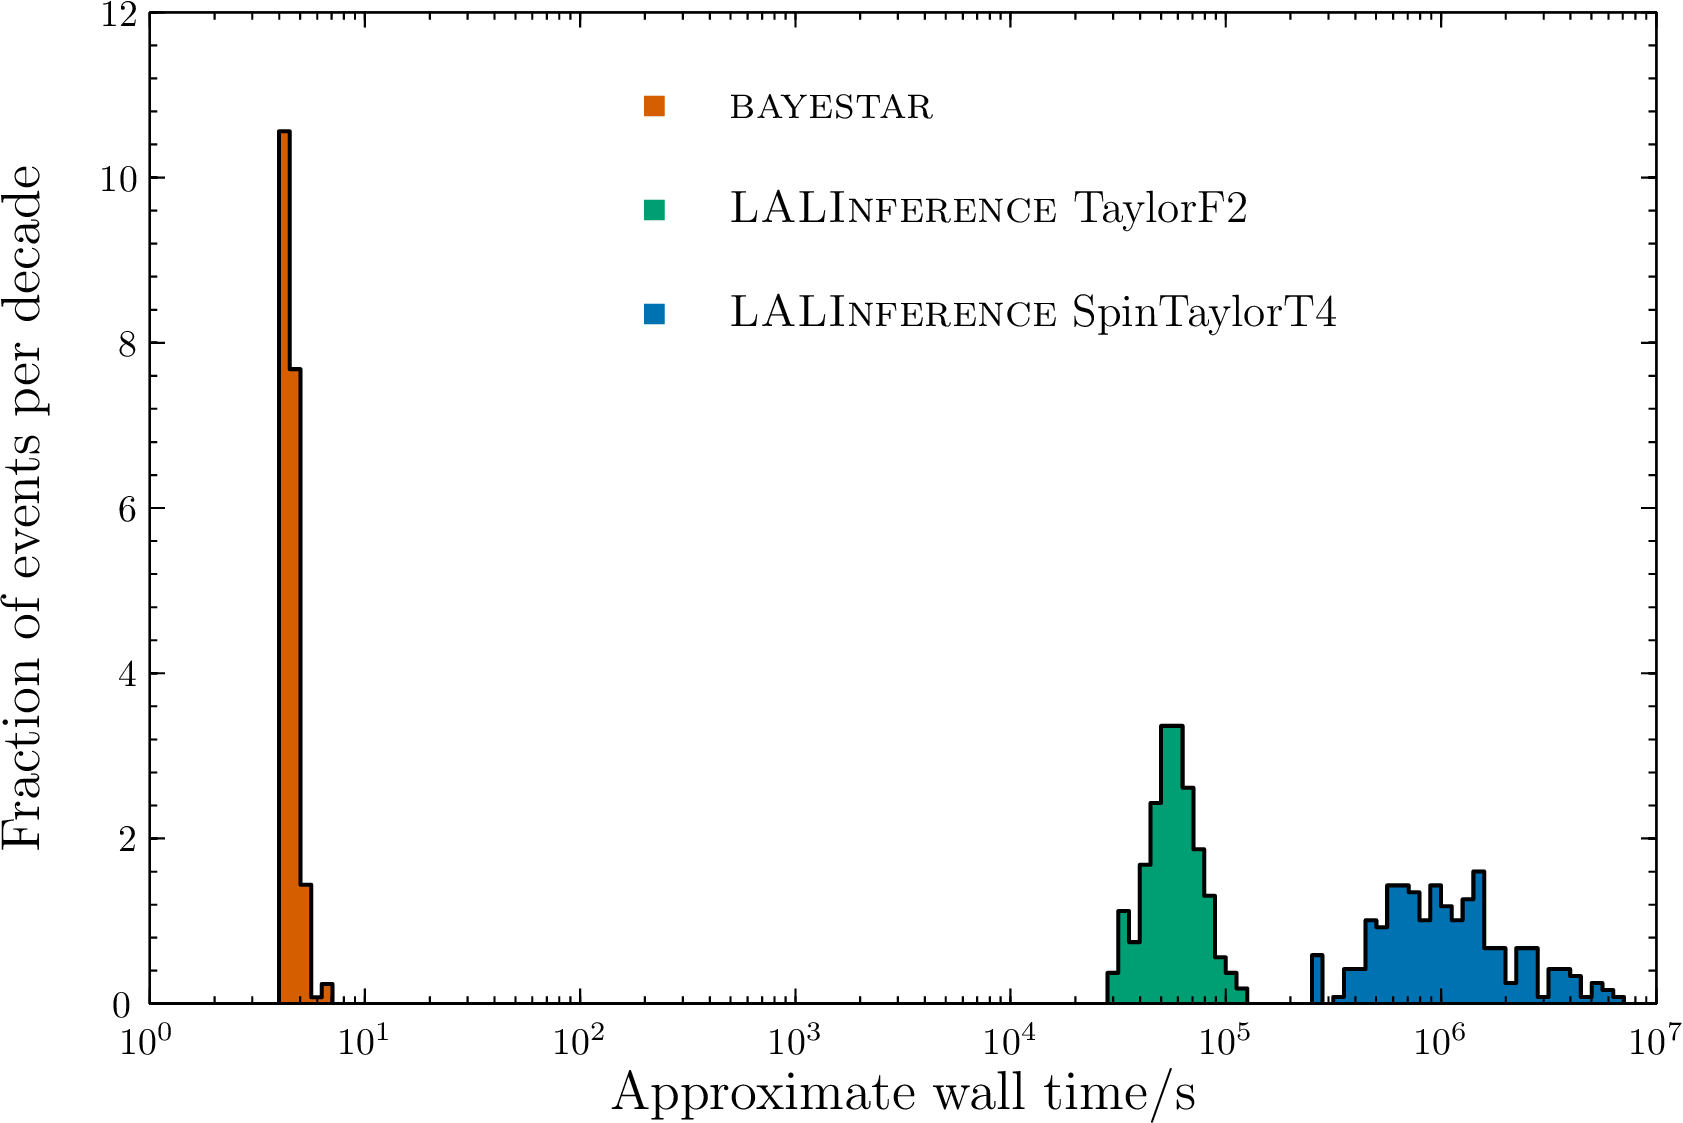
\includegraphics[width=0.95\columnwidth]{figures/Fig_final_time_hist1/Fig_final_time_hist}
  \caption{\protect\label{fig:spinPDFcred} The distribution of one-dimensional marginalized posterior probability density functions (PDFs) of spin magnitudes of the more and less massive components ($\chi_1$ and $\chi_2$, respectively) for all $250$ simulated sources. Shaded regions show the $90\%$ credible boundaries for the spin distributions of the population, and the solid lines show the average of each PDF.  The posteriors have very consistent morphology and span the majority of the prior range.  The spin of the most massive component is typically slightly more constrained toward low values, but even a maximal spin of $\chi_1 = 1$ is rarely ruled out.
  } 
\end{figure}

\bibliographystyle{apj}
\bibliography{bibliography/biblio} 

\end{document}
